\documentclass{article} % For LaTeX2e
% We will use NIPS submission format
\usepackage{nips13submit_e,times}
% for hyperlinks
\usepackage{hyperref}
\usepackage{url}
% For figures
\usepackage{graphicx} 
\usepackage{subfigure} 
% math packages
\usepackage{amsmath}
\usepackage{amsfonts}
\usepackage{amsopn}
\usepackage{ifthen}
\usepackage{natbib}

\title{Project-I by Group CITYNAME}

\author{
Roman Shirochenko\\
Corentin Tallec\\
EPFL \\
\texttt{roman.shirochenko@epfl.ch}\\
\texttt{corentin.tallec@epfl.ch} \\
}

% The \author macro works with any number of authors. There are two commands
% used to separate the names and addresses of multiple authors: \And and \AND.
%
% Using \And between authors leaves it to \LaTeX{} to determine where to break
% the lines. Using \AND forces a linebreak at that point. So, if \LaTeX{}
% puts 3 of 4 authors names on the first line, and the last on the second
% line, try using \AND instead of \And before the third author name.

\nipsfinalcopy 

\begin{document}

\maketitle

\begin{abstract}
	In this report we summarize the results we obtained for the first machine
	learning of the EPFL machine learning course. Facing two datasets, we fit
	linear models and perform linear regression on the first one, and perform data
	classification using logistic regression on the second one. For the first
	dataset, we find that simple linear regression and ridge regression gives
	decent results, but that we can get better results by isolating one simple
	feature and performing transformations on that feature.
\end{abstract}

\section{Linear Regression}
\subsection{Data Description}
Our first data set consisted of a train set, with an input and an output
variable respectively $\mathbf{X}$ and $\mathbf{y}$, composed of $N=2800$ data
samples, and a test set with only $\mathbf{X}$ variable observed and $N=1200$
data samples. $\mathbf{X}$ spans over $D=77$ features, among which 9 of them are
categorical, with number of categories ranging from 2 to 4, 2 of them are binary
and the other are real-valued.

Our goal is to produce linear predictions for test examples and approximate the
test error.

\subsection{Data visualization and cleaning}
The first tasks we performed on the data was to visualize it. The first thing we
did was to obtain a visualization of the data, showed in \ref{fig:boxplotX} and
\ref{fig:histY}. Those two figures led us to normalize both the input and the
output variable (normalizing the output variable allow us to have results that are
easier to interpret, as they are to be compared to values close to 1). No
obvious outliers are noticeable on the $\mathbf{y}$ histogram.

We performed featurewise analysis to notice that most of our real valued
variables have nearly gaussian distributions (or at least unimodal
distributions), which is not the case of our output variable. Figure
\ref{fig:cor1} shows how the output variable evolves as a function of the first
feature. This behaviour is what we notice on most variables, and thus shows no
clear correlations.

Although for variables 49 and 66 we notice a multimodal distribution that is
closer to the behaviour of our output variable, as seen in Figure
\ref{fig:xhist49} and Figure \ref{fig:xhist66}. We thus chose to try and predict
$\mathbf{y}$ using only those two features, transformed through polynomial
transformation.

The categorical variables were encoded using dummy encoding, what led to a total
feature number of 100. As the rank of our dataset is below 100 (it is 70),
simple linear regression is likely to fail, and we use ridge regression to cope
for the rank deficiency.

\begin{figure}[!t]
\center
\subfigure[Boxplot of $\mathbf{X}$.]{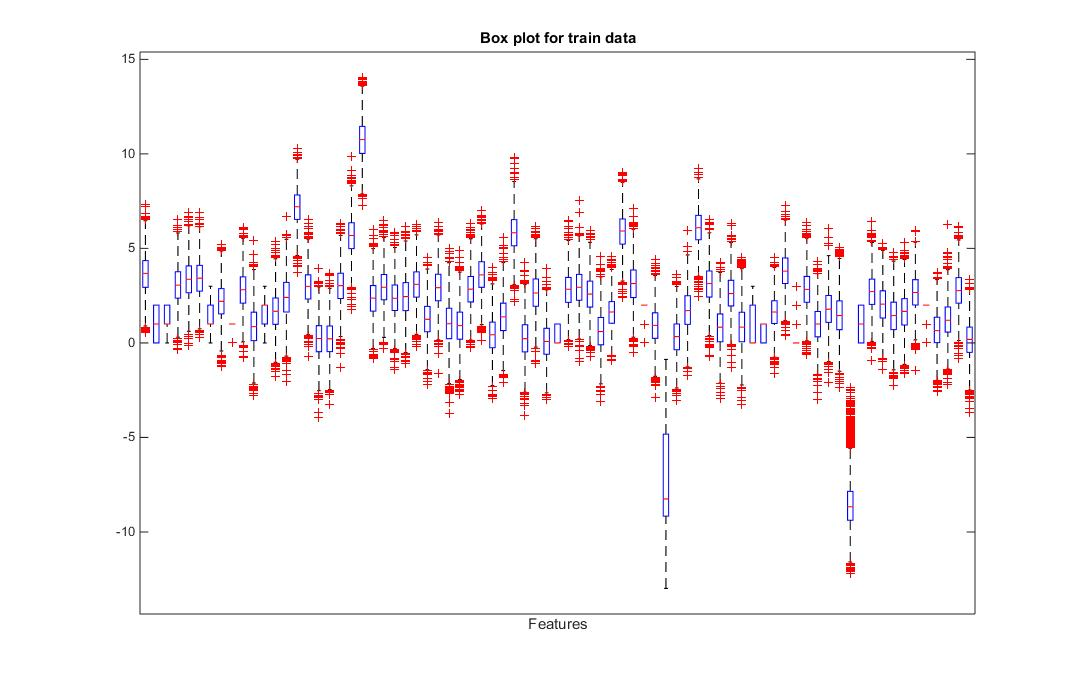
\includegraphics[width=2.5in]{figures/boxplot.jpg} \label{fig:boxplotX}}
\subfigure[$\mathbf{y}$ as a function of the first feature of $\mathbf{X}$.
The correlation between the two variables is not
clear.]{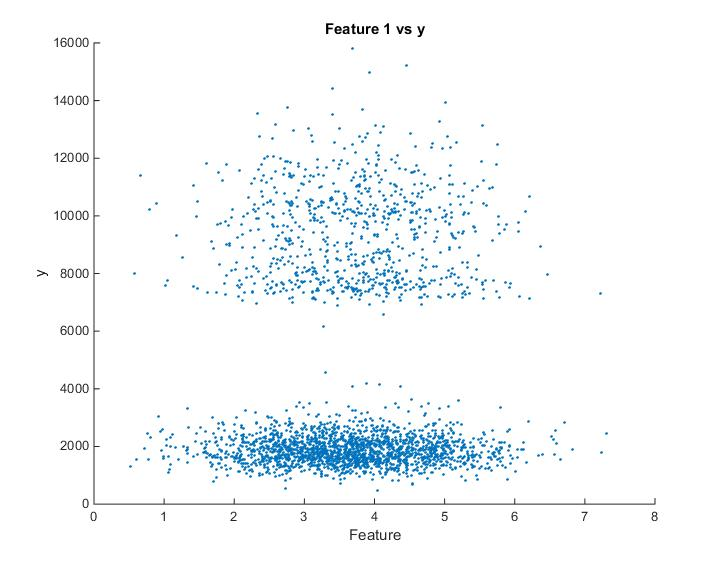
\includegraphics[width=2.5in]{figures/cor1.jpg}\label{fig:cor1}}
\hfill
\subfigure[Histogram of
$\mathbf{y}$. The output distribution is bimodal.]{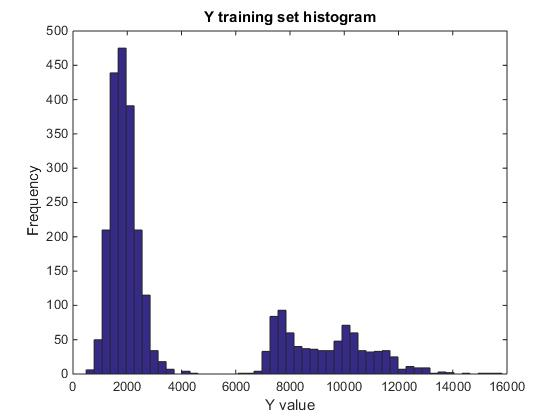
\includegraphics[width=1.5in]{figures/yhist.jpg} \label{fig:histY}}
\hspace*{0.3in}
\subfigure[Histogram of feature 49 of $\mathbf{X}$. We see that the distribution
	is bimodal, as the output.]{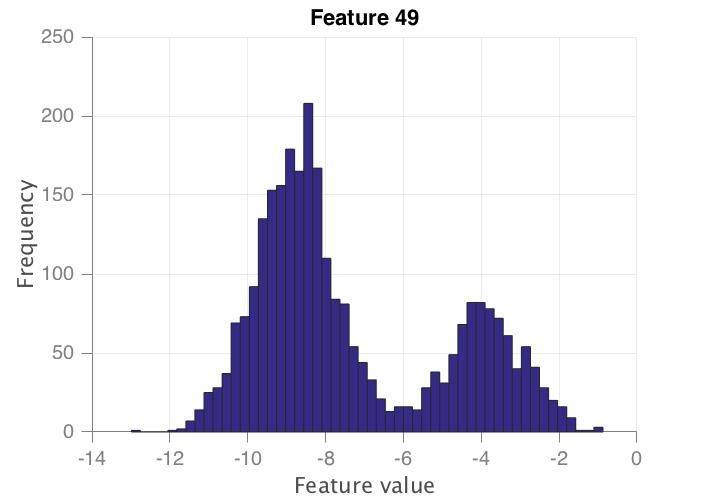
\includegraphics[width=1.5in]{figures/xhist49.jpg}
\label{fig:xhist49}}
\hspace*{0.3in}
\subfigure[Histogram of feature 66 of $\mathbf{X}$. Again, the distribution is
	bimodal.]{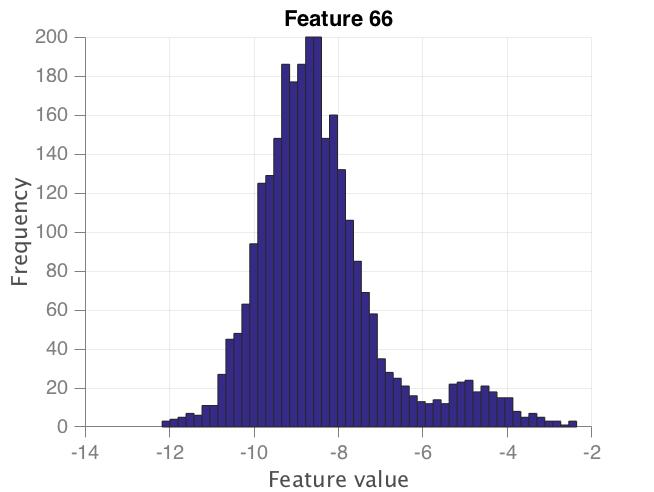
\includegraphics[width=1.5in]{figures/xhist66.jpg}
\label{fig:xhist66}}
\caption{}
\end{figure}

\subsection{Ridge regression}
As the dimension of the data is inferior to the number of feature, we expect
least-squares to work quite poorly, and thus decided to apply mostly ridge
regression.

For our first attempt at predicting the data, we simply used the initial
features and used kFold with $k=4$ to display the evolution of the RMSE as a
function of the regularizing lambda both for the training and test data. 
The lambda we used ranged from $10^{-4}$ to
$10^3$, with 500 points. The results of the ridge regression are already
satisfactory, with an error of approximately $0.105\pm0.001$ on the training set
and $0.115\pm0.001$ on the test set, that is approximately one tenth of the
variance of the output variable.

We see that for sufficiently low lambda, both the training and test errors do
not vary much (there is indeed only a very slight variation of test RMSE, with a
nearly unnoticeable minimum between $\lambda=10$ and $\lambda=100$).

The results described here are summerized in the Figure \ref{fig:ridgeCurve}.

\subsection{Feature transformations}
As notified in a previous section, among all the feature at our disposal,
features 49 and 66 show distributions that ressemble the ditribution of the
output variable. 

This led us to try and regress only on thos two features and polynomial
transformations of them. Using only those two features, we get an RMSE error
that is quite close to the one we notified when all the features are used. When
using polynomial features (up to degree 10), we basically get half the error
that we got using all the features. Those results were obtained using ridge
regression. As in the previous section, we obtained the RMSE as a function of
lambda, calculating both training and test errors using a kFold procedure with
$k=4$. The results are summarized in Figure \ref{fig:polyridgeCurve}, where, as
previously mentionned, we used as features only the two features and their
polynomial transformation with degree ranging from 1 to 10.

This time, the test error varies much more as a function of lambda, and, given
our curve, the best lambda possible seems to be around $10^{-6}$.

Finally to evaluate our performances more accurately, we plotted learning curves
for our model, with 20 features obtained by polynomial transformations and a
lambda of $10^{-6}$. The learning curve is obtained by using $20\%$ of the
training data to perform tests, while learning the model on a progressively
increasing portion of the $80\%$ remaining. We monitor the test and training
error as functions of the proportion of data used to train. The results are
summarized in Figure \ref{fig:learningCurve}. 

As expected, both training error and test error decrease as the proportion of
training data increases. The test error obtained seems to exhibit a quit
satisfactory behaviour.

\begin{figure}[!h]
\center
\subfigure[Ridge regression on kFold with
$k=4$.]{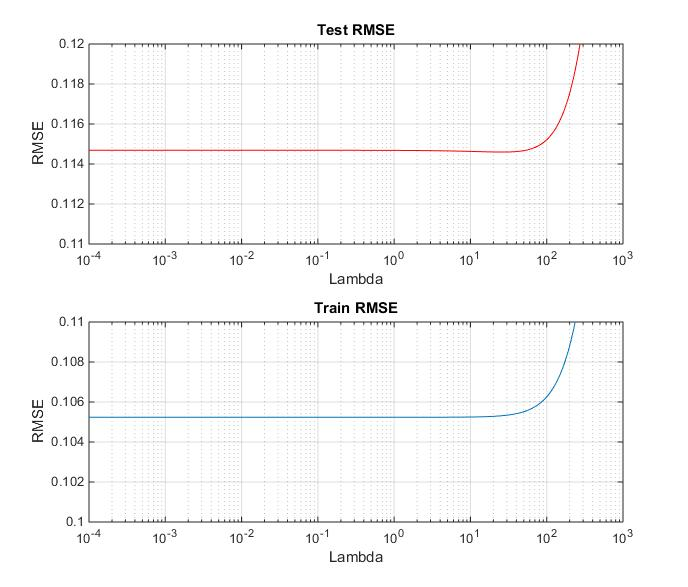
\includegraphics[width=2.5in]{figures/traintestRMSE.jpg} \label{fig:ridgeCurve}}
\hfill
\subfigure[Ridge regression on kFold with feature transformation and
	$k=4$.]{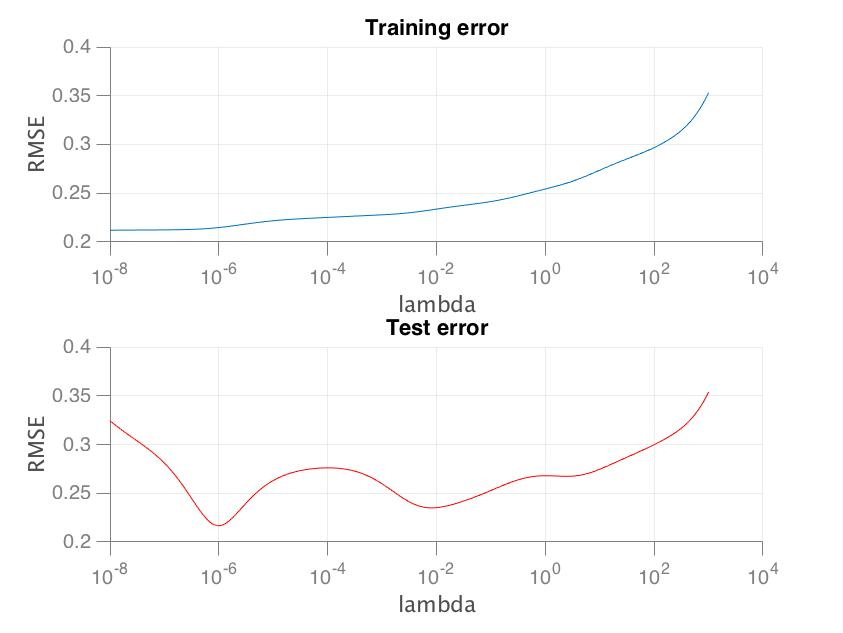
\includegraphics[width=2.5in]{figures/traintestRMSEpoly.jpg}
\label{fig:polyridgeCurve}}
\subfigure[Learning curve. Blue is training data and red is test
data.]{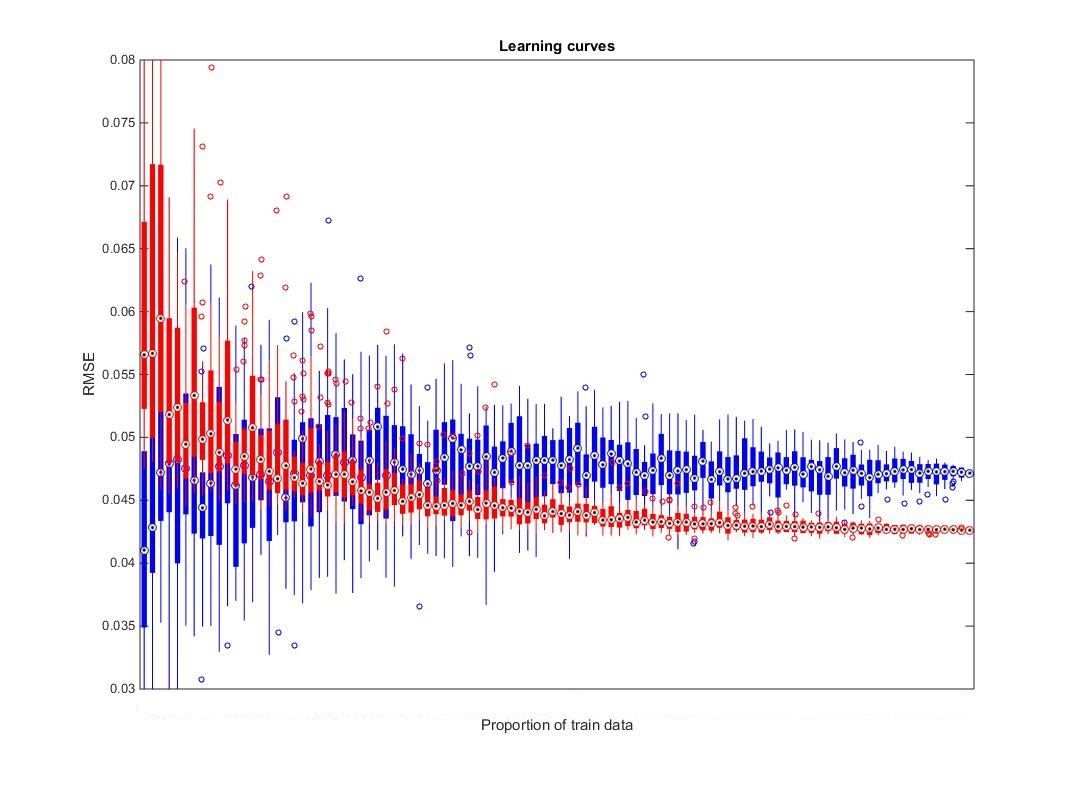
\includegraphics[width=4in]{figures/learningcurves.jpg}
\label{fig:learningCurve}}
\caption{}
\end{figure}


\end{document}
